\section{Udviklingsproces}
Projektforløbet er gennemført over en periode på 4 måneder, hvor der er blevet gjort brug af forskellige arbejdsmetoder og værktøjer. I dette afsnit beskrives hvorledes projektet er gennemført, hvilke metoder der er anvendt samt hvilke udviklingsværktøjer der er benyttet.

\subsection{Gennemførelse}
Under hele projektforløbet har alle gruppens medlemmer arbejdet tæt sammen. Specielt i starten af projektet hvor foranalyse, krav og indledende systemarkitektur blev udarbejdet, arbejdede gruppens medlemmer i tæt fællesskab. 
Da projektet bevægede sig over i detaljeret design og implementering, blev der gjort brug af iterativ udvikling, og gruppens medlemmer blev ansvarlige for forskellige dele. Foruden iterativ udvikling er der også blev udviklet agilt.


\subsubsection*{Iterativ udvikling}
Stort set alle udviklingsprojekter forløber via vandfaldsmodel eller iterativ udvikling. 
Hvis vandfaldsmodellen benyttes gennemløber projektet en række faser, der hver for sig afsluttes, inden næste fase påbegyndes. Opbygning af vandfaldsmodellen kunne eksempelvis være: Krav, analyse, design, implementering og til sidst test.
I et iterativt projektforløb gennemløber projektet i stedet en række iterationer, der hver for sig kan ses som miniudgaver af vandfaldsmodellen. Iterationer, der ligger tidligt i et projektforløb, vil ofte omhandle grundfunktionalitet, mens iterationer senere i projektforløbet bruges til at tilføje funktionalitet til systemet. 

\newpage 

Da systemarkitektur og design er opdelt i use cases, var det oplagt at opdele detaljeret design og implementering  i iterationer. Detaljeret design og implementering opdeles i fire iterationer, og nedenfor beskrives indholdet af de forskellige iterationer.  

\textbf{Iteration 1}\\
I den første iteration er fokus på systemets mest grundlæggende funktionalitet. 
Drone gøres i stand til at oprette forbindelse til server via 3G-shield'et.
Desuden tilsluttes batteri, ESC'er, motorer og ultralyds sensorer til drone. 
Målet med iterationen er at kunne gennemføre use case 1. 

\textbf{Iteration 2}\\
I iteration 2 er hovedformålet at få kommunikation mellem server og drone til at fungere. Bruger skal kunne oprette nye flyveopsætninger og gøre dem tilgængelige på server for dronen. Ydermere skal drone kunne finde egen GPS position, flyvehøjde og orientering. Ud fra viden om egen position, flyvehøjde og orientering skulle dronen kunne flyve til lokationer som er forudbestemt af bruger. Efter denne iteration skal use case 2 og 3 kunne gennemføres.

\textbf{Iteration 3}\\
I iteration 3 er hovedformålet at tilføje billede håndtering. Der monteres kamera på drone, så der kan tages billeder under flyvning. Billeder taget under flyvning sendes via mobilnet fra drone til server og gøres tilgængelige for bruger. Målet med iteration 3 er at kunne gennemføre use case 4 og 5.

\textbf{Iteration 4}\\
Iteration 4's hovedformål var at udvikle antikollision til dronen. Inden tilføjelsen af antikollision kunne dronen udelukkende flyve i lukkede områder uden forhindringer. Tilføjelsen af antikollision skal muliggøre flyvning i normale områder med forhindringer. Efter denne iteration skal alle use cases kunne gennemføres.


\subsubsection*{Agile arbejdsmetoder}
Agil systemudvikling har fokus på løbende at levere værdi til kunden gennem en fleksibel og omskiftelig udviklingsproces. Udvikling og dokumentationen af projektet har forløbet meget agilt. Metoder som scrum light er blevet anvendt, og under construction fasen blev der ofte gjort brug af scrum meetings brugt og backlog til at bevare overblik over projektets fremgang.


\newpage
\subsection{Metoder}
I dette afsnit beskrives de metoder der er blevet benytter i projektet.

\subsubsection*{RUP model}
\textbf{R}ational \textbf{U}nified \textbf{P}rocess er en systemudviklings metode der er blevet anvendt til at definere den overordnede ramme for projektet. RUP er opbygget af de fire faser som beskrives nedenfor.  

\begin{figure}[H]
	\centering
	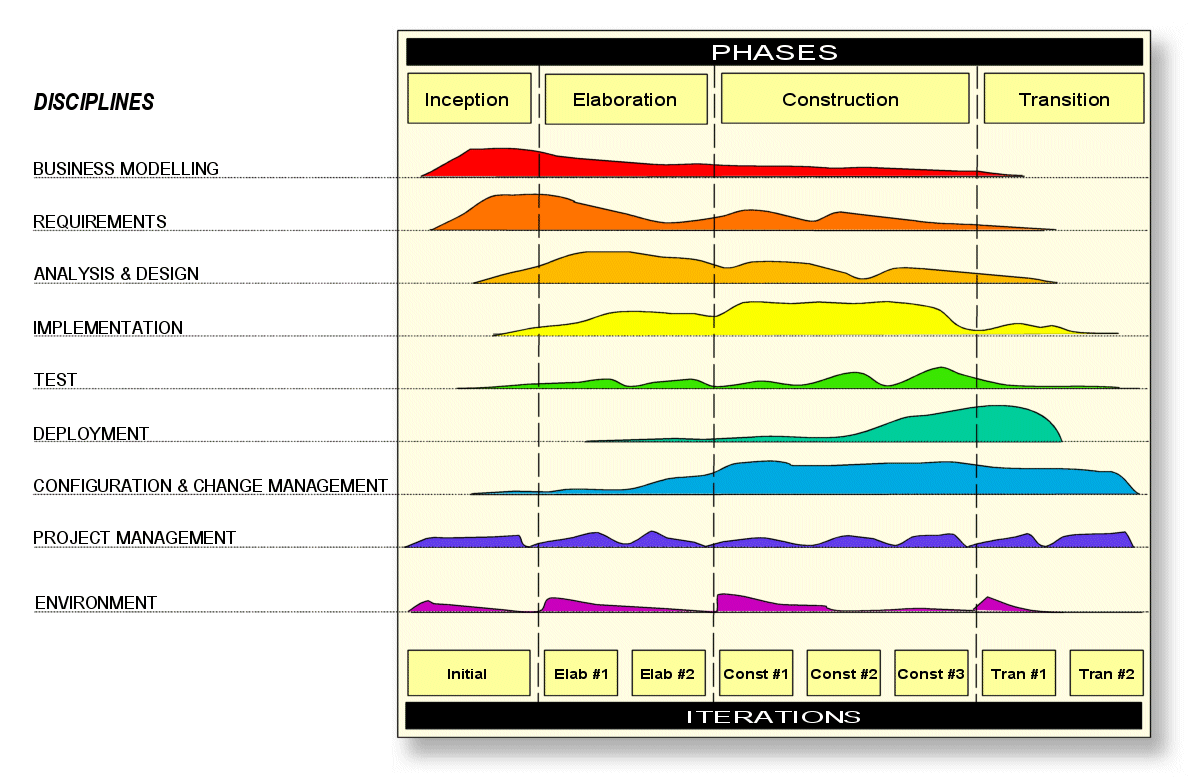
\includegraphics[width=0.80\textwidth]{Billeder/Udviklingsproces/RUP}
	\caption{RUP model}
	\label{fig:rup}
\end{figure}

\textbf{Inception}\\
Inception fasen er projektets indledende fase, og bruges til at lave forundersøgelse, valg af hardware/software samt opsætning af krav. Funktionelle krav opsættes vha. use case analyse af systemets funktionalitet, mens ikke-funktionelle krav er generelle krav til systemspecifikation.
I løbet af inception fasen blev foranalyse, indkøbsliste, krav til systemet og overordnet systemskitse udarbejdet. 

\textbf{Elaboration}\\
Elaboration fasen tager hånd om systemarkitektur og design. I denne fase udarbejdes der indledningsvis en domain model, og derefter laves systemarkitektur for hardware og software. 

\textbf{Construction}\\
I construction fasen er produktet i fokus, og der skiftes løbende mellem implementering af ny funktionalitet, test og dokumentation af nytilføjet funktionalitet. 

\textbf{Transition}\\
Transition er den afsluttende fase, og denne fase tager hånd om færdiggørelse af projekt og overdragelse af produkt. Idet vi ikke har nogen egentlig kunde, bruges afsnittet til lave accepttest, færdiggøre dokumentation og udarbejdelse af rapport. 

\newpage

\subsubsection*{ASE modellen}
ASE modellen som ses på figur \ref{fig:dokument_udvikling} er brugt i kombination med arbejdsmetoden RUP. RUP bruges til at danne overordnede rammer for projektet, mens ASE modellen bruges til definere hvilke dokumenter der skal udarbejdes og hvornår. På figur \ref{fig:dokument_udvikling} vise hvilke dokumenter der oprettes som produkt af ASE modellen. 

\begin{figure}[H]
	\centering
	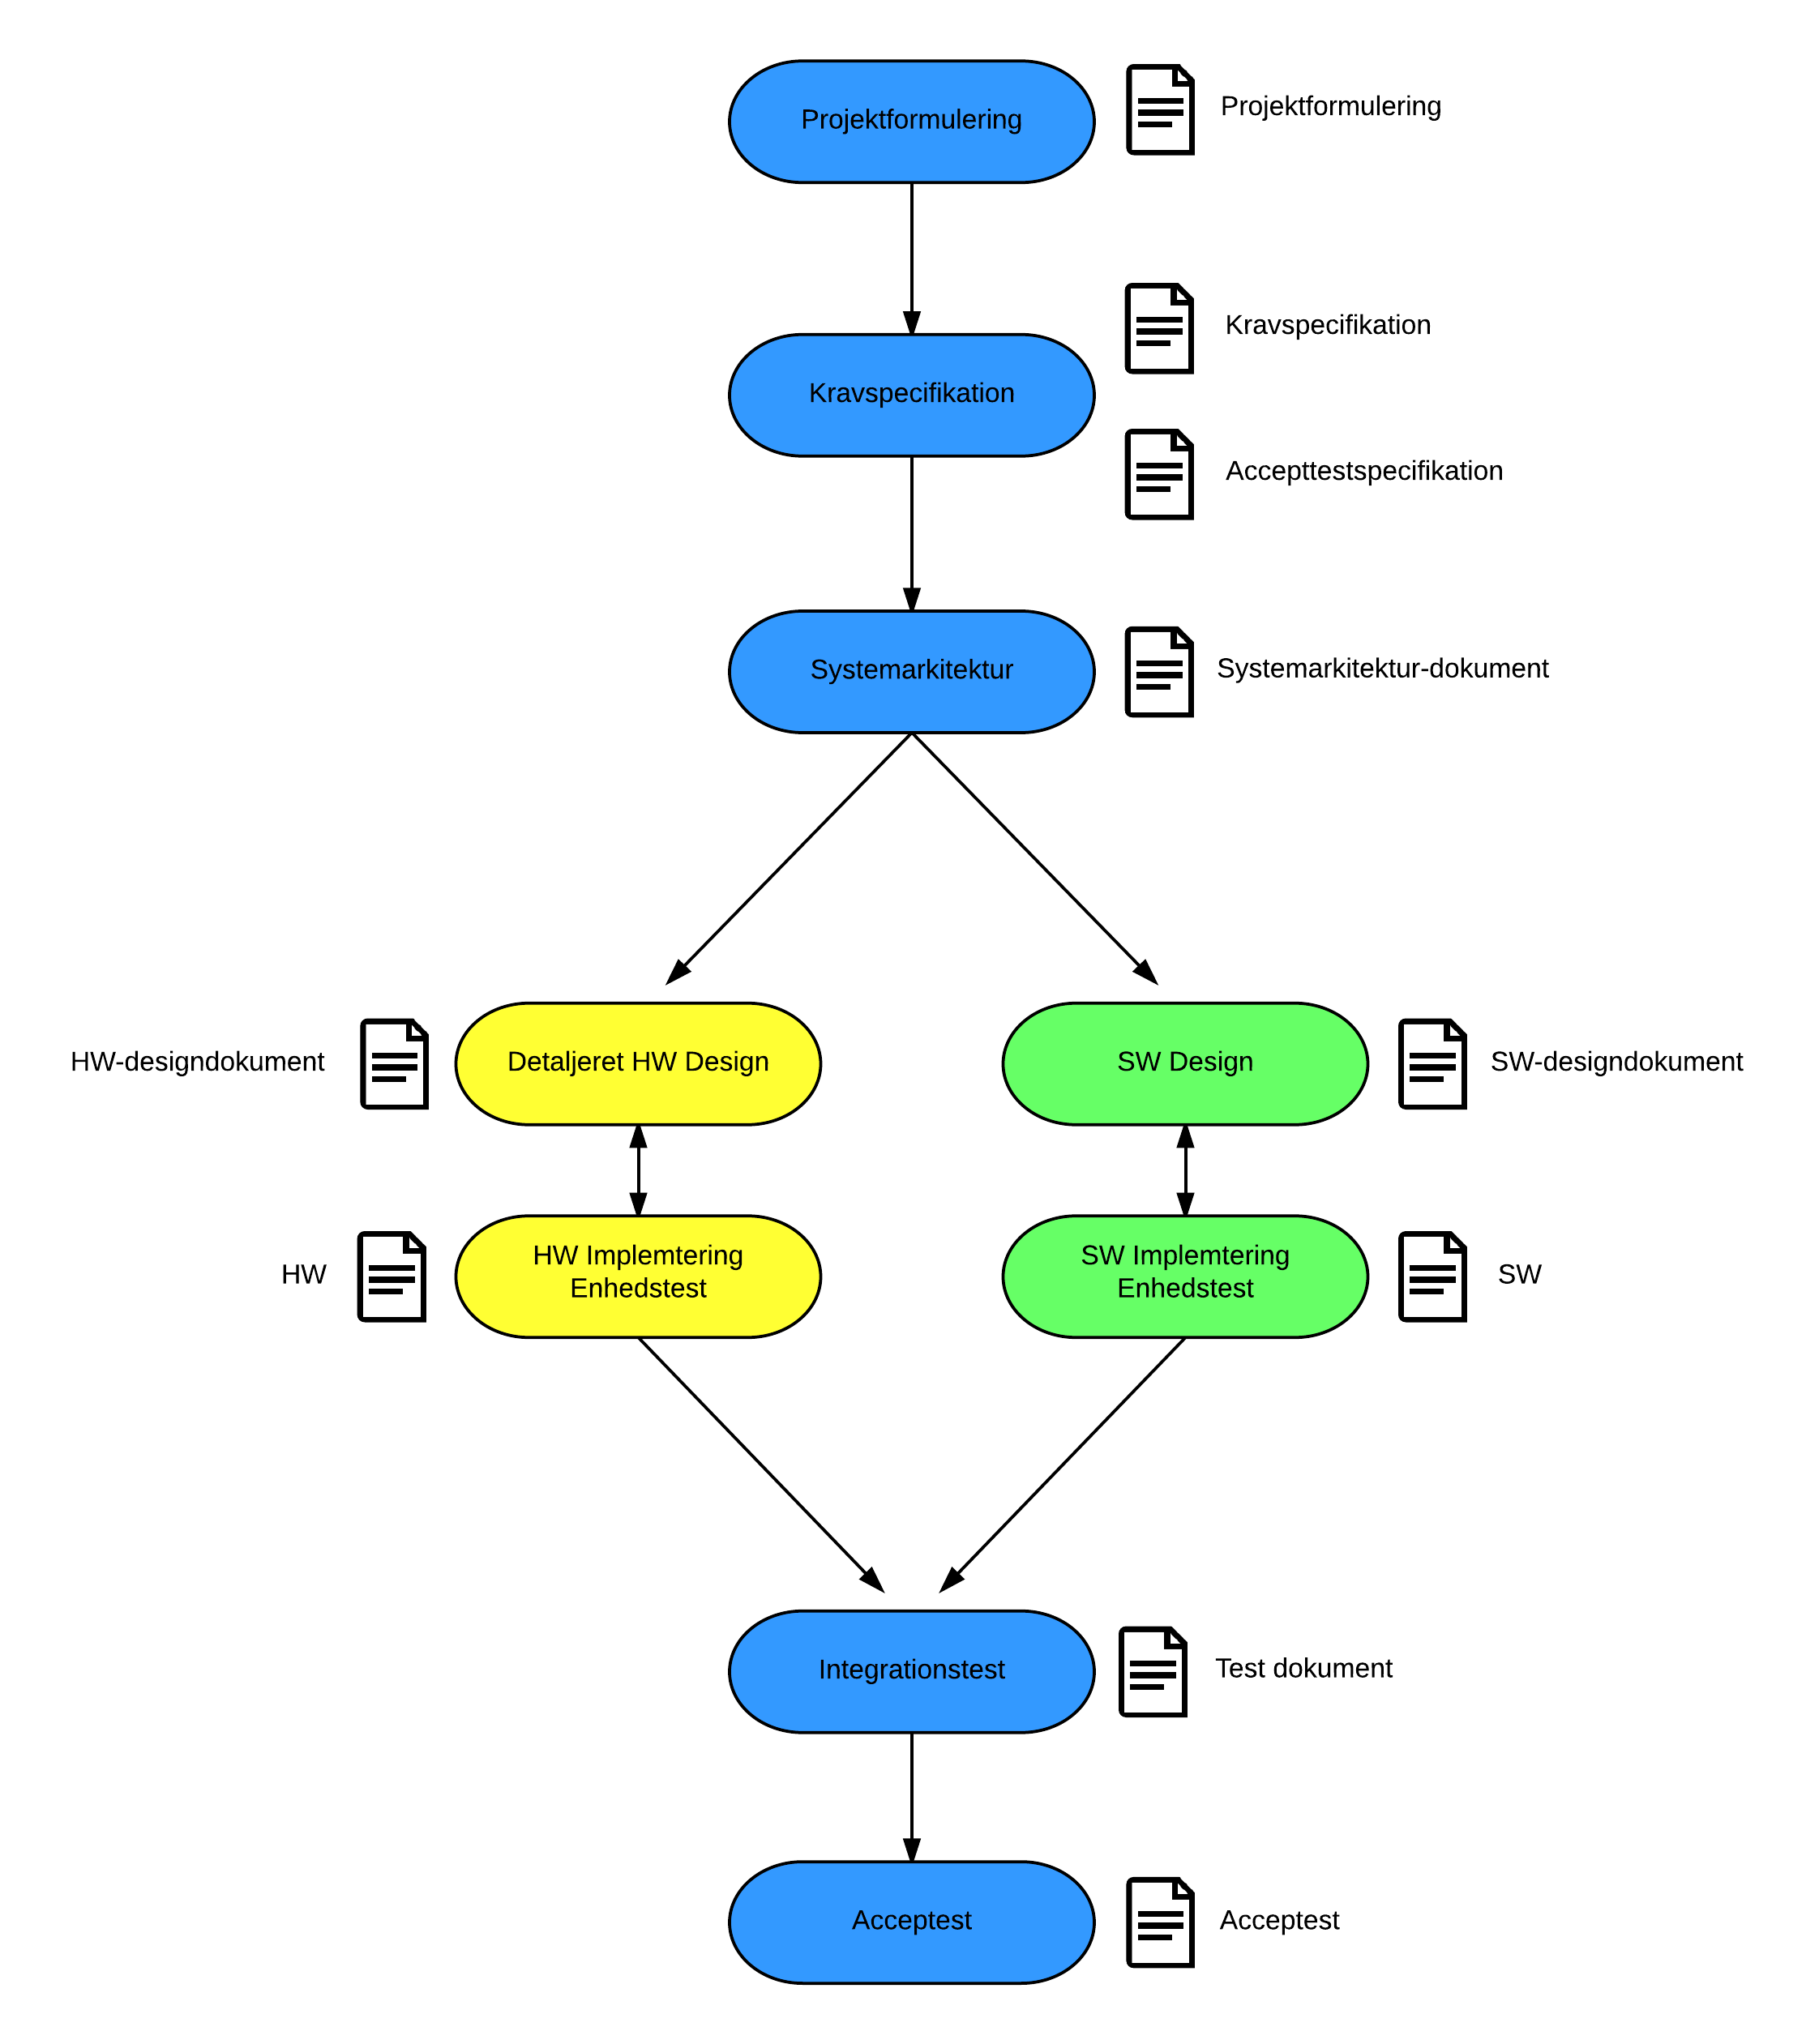
\includegraphics[width=1\textwidth]{Billeder/Udviklingsproces/ase_model}
	\caption{ASE modellen}
	\label{fig:dokument_udvikling}
\end{figure}

\newpage

\subsubsection*{N + 1 model}
Alt software design i projektet er udført ud fra systemudviklings modellen N + 1 [X]. 
Modellen er en udviklingsmodel der beskriver software fra flere forskellige view's.  
Med N + 1 modellen tages der altid udgangspunkt i et use case view. Derefter er det op til udviklerholdet at bestemme hvor mange views der skal bruges for at beskrive systemet på tilstrækkelig vis. 

Til beskrivelse af systemets software anvendes en 5 + 1 view model, som indeholder use case view, logical view, process view, data view, deployment view og implementation view. De nævnte view's beskrives mere uddybende på den følgende side. 

\begin{figure}[H]
	\centering
	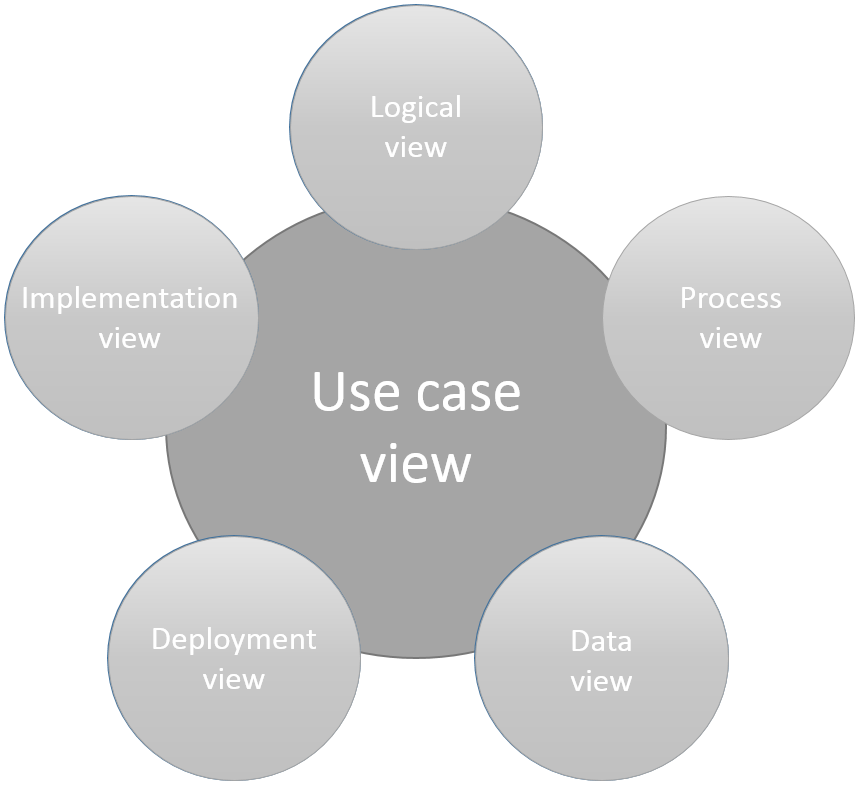
\includegraphics[width=0.7\textwidth]{Billeder/Udviklingsproces/n+1}
	\caption{5 + 1 model}
	\label{fig:n+1}
\end{figure}

\newpage


\textbf{Use case view}\\
Use case viewet består af use case beskrivelser, der er udviklet ud fra brugers synspunkt og som bruges til at beskrive systemets funktionalitet og forskellige brugsscenarier. Alle udarbejdede use case beskrivelser forefindes i kravspecifikationen.

\textbf{Logical View}\\
Logical view bruges til at beskrive de logiske blokke i systemet. På baggrund af hver iteration, er der udarbejdet tilhørende Designoverview-, pakke-, klasse-, sekvens- og state machine diagrammer. Diagrammerne bruges til at give et overblik over systemets funktionalitet på et mere detaljeret niveau.

\textbf{Process View}\\
Process view bruges til at beskrive sideløbende processer/tråde i systemet og hvordan samspillet imellem disse er. I view'et beskrives også krav til timing i kommunikation mellem drone og server.

\textbf{Data View}\\
I data viewet beskrives layout af data der gemmes i systemet og hvordan det lagres. Desuden beskrives hvordan data sendes rundt i systemet og hvordan servers database tilgås.

\textbf{Deployment View}\\
Deployment view beskriver systemets grundlæggende fysiske elementer og sammenspillet mellem dem. I view'et beskrives også hvilke software pakker der bruges i systemet og hvor de bruges. Desuden beskrives hvilke protokoller der er anvendt, fx. layout af meddelelser med header/start/stop

\textbf{Implementation View}\\
Implementation view beskriver vigtige elementer i systemet som ikke er blevet beskrevet i andre views. Bla. beskrives hvilke værktøjer der er benyttet til projektet og hvordan disse værktøjer er sat op. Det beskrives også hvilke filer systemet er bygget af og hvordan disse filer skal linkes sammen.


\newpage
\subsection{Udviklingsværktøjer}
I dette afsnit beskrives de udviklingsværktøjer [X] der er benyttet i løbet af projektet. \\

\textbf{Latex}\\
Latex er benyttet til udarbejdelse af dokumentation og rapport. 

\textbf{Git}\\
Git er versionsstyring og fildelings værktøj.

\textbf{Lucidchart}\\
Lucidchart er benyttet til udarbejdelse af software diagrammer.

\textbf{Visio}\\
Visio er benyttet til udarbejdelse af hardware diagrammer.

\textbf{Atmel studio 6.2}\\
Atmel studio er det IDE hvor kode til main controller skrives.

\textbf{Arduino IDE}\\
Arduino IDE er brugt til at teste kode til main controller.

\textbf{Atom}\\
Atom er et IDE / tekstbehandlings program til håndtering kode.

\textbf{OSX ternimal}\\
Opsætning og programmering af server og webapplikation. 

\textbf{SQLite database}\\
SQLite er benyttet til systemets database.